\documentclass[output=paper]{langsci/langscibook} 
\author{David Wilmsen\affiliation{American University of Sharjah}} 

\title{Extensions and commonalities in negative existential cycles in Arabic}
 

\abstract{The many varieties of Arabic together exhibit numerous existential particles, all of them negated with the usual verbal negator \textit{mā} or occasionally the common Semitic \textit{lā}. A few of those, \textit{ʔys}, \textit{šī}, and \textit{bī}, exhibit stages of a negative existential cycle. All three cycles share commonalities. Associated with an incipient stage A>B, each undergoes a univerbation between the negator and the existential particle. With the \textit{šī} cycle, this involves either reflexes of a fusion between the negator \textit{mā} and \textit{šī} as \textit{māšī}, or a further step involving the negator \textit{mā}, a 3rd-person pronoun \textit{hū} or \textit{hī}, and the existential particle \textit{šī: mā hū/hī šī > mahūš > mūš > muš/miš}. A univerbation of the existential \textit{bī} proceeds along an analogous pathway: from \textit{mā bi} through \textit{mā hū bi > mahub > mub}. As for \textit{ʔys}, it has fused with the negator \textit{lā} to form \textit{laysa}. In all three cycles, these univerbations extend into the domain of equational sentence negation. Another commonality is that as the cycles progress, the original existential particles themselves disappear, to be replaced by new ones. In the \textit{bī} and \textit{šī} cycles, it is the preposition \textit{fī} ‘in’, which has become grammaticalized as an existential particle. In the \textit{laysa} cycle, existential \textit{ʔys} is replaced by demonstratives \textit{hunāka} and \textit{θamma} ‘there’. The univerbations in all three cycles can operate in sub-domains of verbal negation. The stages that the three cycles have reached permit a comparative diachrony. Because the \textit{laysa} cycle is the only one to reach a full-on stage C>A, it must be the longest running, followed by the \textit{šī} cycle, which appears to be entering upon a Stage C in Egyptian Arabic and has done in one southern Yemeni variety. The \textit{bī} cycle, having reached only an incipient stage A>B and beyond would be the most recent.

\textbf{Keywords:} Arabic dialects, Arabic existential particles, Arabic negative existential cycles, Arabic non-verbal negation, Arabic verbal negation 
}

\begin{document}
\maketitle

\section{Introduction} \label{s:WiAR-1}

Extant spoken Arabic varieties exhibit amongst themselves reflexes of at least six separate existential particles. Of these, two show developments characteristic of a negative existential cycle \citep{Croft1991} variously distributed amongst Arabic dialects. For its part, the Arabic of writing, descended from an archaic form, no longer spoken as a native language and different in many ways from the many varieties of spoken Arabic, also shows signs of having passed through a negative existential cycle. We shall summarize the workings of the cycle with each of the three existential particles, observing the commonalities that their cycles share with each other.\footnote{The four other Arabic existential particles (listed in \tabref{tab:WiAR-1} at the start of section 3) show no sign of entering a negative existential cycle.} The stages of completion that these respective cycles have reached will admit proposing a relative chronology.

The first of the cycles to be addressed in \sectref{s:WiAR-2}, is called the \textit{laysa} cycle, after the negator \textit{laysa}, which derives from an existential \textit{ʔys}, no longer in use. The earliest Arabic writing of any length, the Quran, dating to the seventh century, exhibits an early stage of the cycle, with later stages to be seen in collections of the prophetic tradition of the ninth century, in some writings from Muslim Spain of the twelfth century, and subsequent writings, up to the present day.

The second, addressed in \sectref{s:WiAR-3}, is called the \textit{šī} cycle, after an existential particle \textit{šay(y)/šē/šī} of the southern Arabian Peninsula attested in spoken Arabic dialects of the lower Arabian Gulf, Oman, and Yemen. Some original data from Emirati Arabic that will be presented as examples of usage are drawn from a series of oral history recordings, in which pre-nineteen-sixties residents of the old town of Sharjah describe life in the emirate before the oil boom. These are housed at the Sharjah Museums Authority (SMA), acknowledged here with thanks.

The third, addressed in \sectref{s:WiAR-4}, is the \textit{bī} cycle, named for an alternate to the better-known existential particle \textit{fī} of which Croft speaks \citeyearpar[7]{Croft1991}. Some of the data from that discussion are also drawn from the SMA recordings. Statistics pertaining to usage of existential negators involving \textit{bī} come from a corpus of Gulf Arabic (Gumar).\footnote{\url{https://camel.abudhabi.nyu.edu/gumar/}}

Finally, \sectref{s:WiAR-5} addresses some of the salient commonalities that the three Arabic cycles share, placing those into the broader typology of negative existential cycles, there and in the conclusion placing them into a historical perspective.

\section{The \textit{laysa} cycle}
\label{s:WiAR-2}
An existential particle \textit{ʔys} is attested in a few medieval Arabic lexicographical works.
\footnotemark
\footnotetext{The \textit{laysa} cycle is examined in much greater detail in \citet{wilmsen2016a}.} In the earliest of these, the eighth-century Omani lexicographer al-Farahidi (d. 786 AD) says that, in his day, \textit{ʔys} may have fallen out of usage except for a single living idiomatic expression, which he adduces:

\ea \label{ex:WiAR-1}
	\gll ʔat-ni b-h mn ḥyθ ʔys w lys \\
	come.\textsc{pvf} \textsc{prep-pro.3msg} \textsc{prep} \textsc{adv} \textsc{exist} \textsc{conj} \textsc{nex}\\
	\glt `He came [to] me with him/it from wherever. (lit. where there and not there)' \citep[105]{al-far2003a}
\z

al-Farahidi remarks that \textit{ʔys} denotes existence, and \textit{lys}, which he derives from \textit{lā ʔys}, denotes nonexistence. Some ninth-century Arabic philosophical writing uses the two with those meanings \citep[35]{gihami-a}. Soon afterwards, the affirmative existential particle \textit{ʔys} disappears from living usage, leaving the negative \textit{laysa} abundantly attested in the Arabic of writing from that day to this. Consequently, we may assume that an existential particle \textit{ʔys} did once obtain in some varieties of Arabic and it that was negated with the common Semitic negator \textit{lā}:\footnote{Other Semitic languages possess similar existential particles, with some, including Arabic, retaining only the negated form. Their origins are much discussed and debated amongst Semiticists. Nevertheless, despite some disagreement around the derivation of \textit{laysa} \citep{wilmsen2016a, al-jallad2018a}, a plurality consensus holds that it does, indeed, derive from \textit{lā ʔys} (see \citet{blau1972a, gensler2000a}, \citet[464--465, 488--489]{lipi2001a};summarized in \citet[329--331]{wilmsen2016a} \& \citet[298--299]{wilmsen2017a}.}

\ea \label{ex:WiAR-2}
	\gll lā ʔys\\
	\textsc{neg} \textsc{exist}\\
	\glt `Not there [is]’\footnote{In Arabic, a copula is usually not expressed in present time predications. The enclosing of the English copula in brackets in the gloss is meant to reflect that. } \citep[105]{al-far2003a}
\z

The regular Arabic verbal negator, \textit{lā}, negating an existential particle, makes this a characteristic type A construction, in which, as Croft defines it, “there is no special existential negative form, and the negative existential construction is the positive existential predicate plus the ordinary verbal negator” \citeyearpar[6--7]{Croft1991}. In the Arabic of writing, verbal negations almost always proceed with a reflex of \textit{lā} (sometimes \textit{mā}):

\ea \label{ex:WiAR-3}
	\gll lā a-ʕraf \\
	\textsc{neg} \textsc{1sg}-know.\textsc{ipfv} \\
	\glt ‘I [do] not know.’ \citep[144, 158]{adwan2000a}
\z

\subsection{Stage A>B of the \textit{laysa} cycle} \label{s:WiAR-2.1}

Croft continues, defining a stage A>B as involving “a special existential negative form, usually but not always a contraction or fusion of the verbal negator and the positive existential form” \citeyearpar[7]{Croft1991}. This is what the surviving negative existential particle \textit{laysa} is. A Stage A>B would have seen a conventional negation of existential \textit{ʔys} with \textit{lā}, as that in example (\ref{ex:WiAR-1}), coexisting with \textit{laysa}. That may have happened before Arabic became fully attested in writing, but there is no remaining record of it. Nevertheless, \textit{laysa} can stand by itself in denying the existence of something, to the extent that the thing denied need not be mentioned. In modern writing, this holds especially for negating locational sentences of the type, ‘At/for/in/with the X is/are Y’ (\ref{ex:WiAR-4}a). Nor is \textit{laysa} the sole negator of existential predications; the regular negator \textit{lā} also negates them without the need for an expressed existential particle (\ref{ex:WiAR-4}b):\footnote{The examples of usage with \textit{laysa} are from written sources, meaning that geographical provenance is largely irrelevant. A map charting the spoken Arabic dialects that are passing through negative existential cycles that are addressed below can be found in \figref{fig:ArabicVarieties}}

\ea \label{ex:WiAR-4}
  \ea
  	\gll laysa fī l-maktab illā anā w anta\\
  	\textsc{nex} \textsc{prep} \textsc{det}-office \textsc{conj} \textsc{pron.1sg} \textsc{conj} \textsc{pron.2msg}\\
  	\glt ‘There [is] not in the office except you and I.’ \citep[273]{adwan2000a}
  \ex
  	\gll lā ilāha illā llāh\\
  	\textsc{neg} god except Allah\\
  	\glt ‘[There is] no god except Allah.’ (Quran 37:35)
\z \z

As such, \textit{laysa} does function as a special negative existential form in certain types of existential negations, whereas the usual negator \textit{lā} can also negate existential predications, albeit without need for an expressed positive existential. This would be a type of a stage A>B.

\subsection{Extension into equational sentence negation} \label{s:WiAR-2.2}

Aside from that, \textit{laysa} also negates non-verbal predications of all sorts, whether existential or otherwise. This has been the case at least since the 7th century AD, when extensive Arabic writing began to appear:

\ea \label{ex:WiAR-5}
  \ea
  	\gll laysa ka-miθli-hi šayʔ\\
  	\textsc{nex} \textsc{prep}-likeness-\textsc{pron.3msg} thing\\
  	\glt ‘There [is] not [a] thing like His likeness.’ (Quran 42:11)
  \ex
  	\gll laysa ð-ðakaru ka-l-ʔunθā\\
  	\textsc{neg} \textsc{det}-male \textsc{prep-det}-female\\
  	\glt ‘The male [is] not like the female.’ (Quran 3: 36)
\z \z



Sentences of the type in (\ref{ex:WiAR-5}) are what Li and Thompson call “equational sentences … in which an identificational or member/class relationship is expressed between two NPs” \citeyearpar[419]{li1977a}. That is, equational sentences express relationships between the subject and predicate that in languages like English, French, and Spanish require a copula. Equational sentences are characteristic non-verbal predications in spoken and written Arabic alike, in which a copula, verbal or otherwise, is lacking. When a copula is needed, it is usually one of the 3rd-person pronouns \citep[431--433]{li1977a}:\footnote{For more on equational sentences and the copular function of 3rd person pronouns in Arabic, see \citet{eid1983a, eid1991a} and \citet{choueiri2016a}.}

%\todo{are both examples palestinian arabic or just the first?}
\ea Palestinian Arabic \citep[431]{li1977a}\label{ex:WiAR-6}\\
  \ea
  	\gll hiyye le-mʕallme\\
  	\textsc{pro.3fsg} \textsc{det}-teacher\\
  	\glt‘She [is] the teacher.’
  \ex
  	\gll il-bint hiyye le-mʕallme\\
  	\textsc{det}-girl \textsc{pro.3fsg} \textsc{det}-teacher\\
  	\glt ‘The girl [is] the teacher.’
\z \z

\citet[420]{li1977a} label sentences of the first type (\ref{ex:WiAR-6}a) “topic-comment constructions” and the second “subject-predicate constructions”, noting that both Hebrew, and Palestinian Arabic (among other languages) have developed a copula by means of the topic-comment construction. In actuality, what holds for Palestinian Arabic holds, with minor variations, for all varieties of Arabic: when a copula is needed, it is expressed as a 3rd person pronoun. As far as written Arabic is concerned, topic-comment and subject-predicate constructions alike are characteristically negated with \textit{laysa}, while verbal predications are negated with reflexes of \textit{lā}, as in (\ref{ex:WiAR-3}). 

\subsection{Subsequent stages of the \textit{laysa} cycle} \label{s:WiAR-2.3}

A stage B, which would see “only a special negative existential form” \citep[9]{Croft1991}. Veselinova (\citeyear[1338]{Veselinova2014}; \citeyear[153]{Veselinova2016}) observes that stages of the cycle, especially a stage B, may be skipped entirely, and it appears that the \textit{laysa} cycle has done so. Occasionally, however, \textit{laysa} can negate verbs, characteristic of a stage B>C \citep[9--10]{Croft1991}, and when it does, it is usually for pragmatically marked purposes, notably in posing contrasts between a denial and an assertion (\ref{ex:WiAR-7}a) or in rhetorical negations (\ref{ex:WiAR-7}b), as in the following from an early genre of Arabic literature, collected sayings of the prophet Muhammad (\textit{Hadith}) compiled by \citet[d. 870]{al-bu2000a}:

\ea \label{ex:WiAR-7}
  \ea
  	\gll laysa ya-riθ-u-ni ʔillā ʔibnat-i\\
  	\textsc{nex} \textsc{3m}-inherit.\textsc{ipfv-ind-pron.1sg} except daughter-\textsc{pron.1sg}\\
  	\glt ‘None inherits [from] me except my daughter.’ \citep[Vol. VIII p. 151]{al-bu2000a}
  \ex
  	\gll a laysa ʔamara-kum\\
  	\textsc{q} \textsc{nex} command.\textsc{pfv-pron.2mpl}\\
  	\glt ‘[Has] he not commanded you?’ \citep[Vol. VI p. 864]{al-bu2000a}
\z \z

In (\ref{ex:WiAR-7}a), the predication might still be read as an existential negation: ‘There is none inherits from me.’ Nevertheless, \textit{laysa} can occasionally negate verbs in apparently unmarked usage:\footnote{A rarity in other spoken varieties of Arabic, reflexes of \textit{laysa} survive as what \citet[26]{holes2006a} calls a “fossilized remnant” in some southern Peninsular dialects of Arabic, where they can negate verbal predications \citep[142--144]{al-azraqi1998a}, typical of a stage B>C.}

\ea \label{ex:WiAR-8}
	\gll laysa ya-drī kayfa ħadaθa al-ʔamr \\
	\textsc{neg} \textsc{3m}-know.\textsc{ipfv} \textsc{adv} happen.\textsc{pfv} \textsc{det}-thing\\
	\glt ‘He knows not how the thing happened.’ \citep[28]{kanafani2006a}
\z

Because the negation in (\ref{ex:WiAR-7}) and other verbal negations with \textit{laysa} would usually be effectuated with a reflex of \textit{lā}, the choice to negate the verb with \textit{laysa} must invest the statement so produced with some added pragmatic meaning.

As for a Stage C, “in which the negative existential form is the same as the ordinary verbal negator” \citep[11]{Croft1991}, the \textit{laysa} cycle reached it only in the extinct 12th century Arabic dialect(s) of Muslim Iberia (Al-Andalus), where reflexes of \textit{laysa} had become, “an almost universal negator of the perfective, … imperfectives, and nominal sentences” \citep{corriente2013a}:

\ea \label{ex:WiAR-9}
  \ea
  	\gll las kān dara-yt-uh\\
  	\textsc{nex} be.\textsc{pfv.3s} know.\textsc{pfv-1s-pron.3m}\\
  	\glt ‘I had not known it.’ \citep[126]{corriente2013a}
  \ex
  	\gll las ni-sammī aḥad\\
  	\textsc{nex} \textsc{1s}-name.\textsc{ipfv} one\\
    \glt ‘I mention not anyone.’ \citep[126]{corriente2013a}
  \ex
  	\gll las niḥun ṣibyān\\
  	\textsc{nex} \textsc{pron.1pl} children\\
  	\glt ‘We [are] not children.’ \citep[126]{corriente2013a}
\z \z

\subsection{Terminal stage of the \textit{laysa} cycle} \label{s:WiAR-2.4}

Nevertheless, \textit{laysa} has everywhere entered upon a Stage C>A, “in which the negative-existential-cum-verbal-negator begins to be reanalyzed as only a negator, and a regular positive existential … comes to be used with it in the negative existential construction” \citep[12]{Croft1991}.\footnote{Croft actually says “a regular positive existential verb” \citep[12]{Croft1991}. But in Arabic, the existential particles are almost always not verbs. For its part, \textit{laysa} exhibits the peculiar quality of inflecting as a perfective verb to negate present-time predications. There is no sign that it ever existed in an imperfective form (see discussion in \citealt[341--346]{wilmsen2016a}).} In the Arabic of writing especially, two existential particles \textit{θamma} and \textit{hunāka}, both meaning ‘there’, and a passive-voice construction involving the verb \textit{ya-ǧid} ‘he finds’ > \textit{y-ūǧad} ‘it [is] found’ appear in the 8th and 9th centuries \citep[354–356]{wilmsen2016a}. The usual verbal negator \textit{lā} most often negates the verb form: \textit{lā y-ūǧad} (lit. ‘it [is] not found’ understood to mean ‘there is not’; example [10a]). Otherwise, \textit{laysa} negates the two existential particles, as in the following from the Hadith collections of \citeauthor{anbal-a} (d. 855) and \citeauthor{al-bu2000a} (\ref{ex:WiAR-10}b \& \ref{ex:WiAR-10}c):

\ea \label{ex:WiAR-10}
  \ea
  	\gll fa-lā y-ūǧad fī-hi šayʔ\\
  	\textsc{conj-neg} \textsc{3msg}-found.\textsc{ipfv}	\textsc{prep-pro.3msg} thing\\
  	\glt ‘And there [is] not in it [a] thing.’ [lit. ‘And not found in it thing’] \citep[Vol. VIII p. 1256]{al-bu2000a}
  \ex
  	\gll laysa θamma dinār wa-lā dirham \\
  	\textsc{nex} \textsc{exist} currency \textsc{conj-neg} currency \\
    \glt ‘Not there [is] [a] dinar and not [a] dirham.' \citep[Vol. VIII p. 1323]{al-bu2000a}
  \ex
  	\gll laysa hunāka dinār wa-lā dirham \\
  	\textsc{nex} \textsc{exist} currency \textsc{conj-neg} currency\\
  	\glt ‘Not there [is] [a] dinar and not [a] dirham.’ \citep[Vol. IX, p. 507]{anbal-a}
\z \z

Both of the latter two existentials, originate as remote demonstrative pronouns, corresponding in usage to English ‘there’. In the earliest extensive Arabic writing, the Quran, dating to the middle seventh century, \textit{θamma} appears once as an existential particle, but a reflex of \textit{hunāka} appears only as a demonstrative. Negation of either with \textit{laysa} begins to appear in writing after the middle of the ninth \citep[354--355]{wilmsen2016a}. The \textit{laysa} cycle had thus passed through all of its stages by that time.

It can rightly be asked why all stages of the \textit{laysa} cycle appear to be stacked one atop the other. In the first place, Croft himself notes the overlap of stages (\citeyear[22]{Croft1991}; c.f. \citealp[146, 149, 151--154]{Veselinova2016}). In the second, the Arabic of writing was codified in the eight through tenth centuries and has changed but little since then, such that Arabic texts produced in the eighth century remain intelligible to readers today, and modern writers adhere to their modes of expression \citep[340]{wilmsen2016a}. As it stands, the \textit{laysa} cycle is not likely to proceed further, with \textit{laysa} becoming the regular negator, precisely because of the archaic character that its users cultivate to the present day, tolerating but little deviation from it. Noteworthy, too, is that \textit{laysa} is used in writing but hardly ever in speech.

\section{The \textit{šī} cycle}\label{s:WiAR-3}

For their parts, spoken varieties of Arabic possess between themselves several existential particles \citep{eid2008a}.\footnote{The \textit{šī} cycle is examined at greater length in \citet{wilmsen2020a}.} These are listed in \tabref{tab:WiAR-1}:

\begin{table}[h]
	\centering
	\caption{Existential particles in spoken Arabic varieties}
	\label{tab:WiAR-1}
\begin{tabularx}{\textwidth}{llQ}
\lsptoprule
\textbf{Existential particle} & \textbf{Negation} & \textbf{Provenance} \\ \midrule
\textit{aku} & \textit{mā-kū(-š)} & Iraq, Kuwait, Bahrain \\
\textit{bī} & \textit{mā bī(-š)} & Syrian steppes, central/southern Arabian Peninsula \\
\textit{fī} & \textit{mā-fī(-š)} & Libya, Egypt, Levant, Arabian Peninsula/Gulf \\
\textit{kāyen} & \textit{mā-kāyen-š} & Morocco, Algeria \\
\textit{šī} & \textit{mā šī} & Bahrain, UAE, Oman, Yemen \\
\textit{θamma, famma, emm} & \textit{mā (θ/f)ammā-š, mem-š} & Tunisia, Malta \\ \lspbottomrule   
\end{tabularx}
\end{table}

Most dialects of Arabic possess only one existential particle, but the Arabic varieties of the southern Arabian Peninsula are remarkable for the presence of multiple particles. Bahrain has \textit{aku, fī}, and \textit{šay} \citep[110]{holes2016a}; the Yemen has \textit{šī, fī}, and \textit{bī} \citep[346–348, maps 136 \& 137]{behnstedt2016a}; and Oman and the UAE possess both \textit{fī} and \textit{šī} – the latter variously realized as \textit{šayʔ, šayy, šē}, or \textit{šī} (\citealp[112]{reinhardt1894a}; \citealp[170]{johnstone1967a}; \citealp[24]{brockett1985a}; \citealp[71]{holes1990a}; \citealp[24--28]{holes2016a}; \citealp[162]{davey2016a}). All of these are negated with the negator \textit{mā} common to all spoken dialects of Arabic, which, characteristic of a stage A, negates verbal predications and non-verbal existential predications alike. Indeed, \citep[7]{Croft1991} adduces usage from Syrian Arabic as an example of a stage A. Compare Croft’s examples with an almost identical matched pair from Emirati Arabic:

\ea Emirati Arabic (Sharjah)\label{ex:WiAR-11}\\
  \ea
  	\gll mā a-ʕraf ism-ǝ\\
  	\textsc{neg} \textsc{1sg}-know.\textsc{ipfv} name-\textsc{pro.3msg}\\
  	\glt ‘I know not its name.’ (SMA data)
  \ex
  	\gll mā šay biyūt\\
  	\textsc{neg} \textsc{exist} houses \\
  	\glt ‘There [were] no houses.’(SMA data)
\z \z

For its part, the existential particle \textit{fī} has not proceeded beyond Stage A, but existential particle \textit{šī} has. In Emirati Arabic, \textit{šī} shares the existential function with \textit{fī}:

\ea Emirati Arabic (Sharjah)\label{ex:WiAR-12}\\
	\glll mā šī fayda\\
	\textit{mā} \textit{fī} \textit{fayda}\\
	\textsc{neg} \textsc{exist} benefit\\
	\glt ‘There [is] no benefit.’ (SMA data)
\z

A contrast in usage obtains between the two particles in their affirmative and negative functions in Emirati Arabic. \citet[528]{wilmsen2020a} had observed from limited data that the negation \textit{mā šī} occurs about twice as often as the affirmative \textit{šī} and that affirmative existential predication occurs more often with \textit{fī} than with \textit{šī}. The SMA recordings, from which some of the data for the current study come, reveal a more precise view of the matter. In them, speakers who have occasion to use existential predications use a reflex of \textit{māši} in negation 90 times, as opposed to 32 with \textit{mā fī}. To the contrary, they use \textit{fī} in affirmative existential predication 34 times as opposed to their using \textit{šī} in the affirmative only six times, with some speakers not using it at all. That is, full 85 percent of existential predications are with \textit{fī} and 72.8 percent of existential negations are with a variant of \textit{māši}.\footnote{A similar situation obtains in Yemeni Dialects of Arabic, in which, as Behnstedt observes, “the negative form may differ from the positive one in its base lexeme … such as \textit{bū} ‘there is’, \textit{mā šī} ‘there is not’ \citeyearpar[345]{behnstedt2016a}. We shall return to existential \textit{bī} below.} These figures are summarized in \tabref{tab:WiAR-2}.

\begin{table}[!h]
	\centering
	\caption{Occurrences of Emirati existentials and their negations in SMA oral histories}
	\label{tab:WiAR-2}
\begin{tabularx}{\textwidth}{Qrrrr}
\lsptoprule
\textit{} & \textit{šī} & \textit{fī} & \textit{māšī} & \textit{mā fī} \\ \midrule
Speaker 1F & 0 & 0 & 25 & 4 \\
Speaker 2F & 3 & 1 & 21 & 5 \\
Speaker 1M & 0 & 10 & 18 & 8 \\
Speaker 2M & 2 & 13 & 17 & 7 \\
Speaker 3M & 1 & 5 & 6 & 4 \\
Speaker 4M & 0 & 5 & 3 & 4 \\ \midrule
Totals & 6 & 34 & 90 & 32 \\ \midrule
Percentages & 15 & 85 & 72.8 & 26.2 \\ \lspbottomrule   
\end{tabularx}
\end{table}

\subsection{Stage A>B of the \textit{šī} cycle} \label{s:WiAR-3.1}

Such alternation in usage is in accordance with Croft’s conception of Stage A>B, in which “a special negative existential form is found … in addition to the regular existential form” \citeyearpar[7]{Croft1991}. In this case, the regular existential form being precisely the \textit{fī} that he adduces, albeit for the Syrian Arabic of Damascus. So, too, are univerbations between the negator and the existential particle common in a stage A>B, the negator so formed existing side-by-side with the regular negator + existential particle construction. Existential \textit{šī} does form a univerbation with the negator \textit{mā} to form \textit{maši}. In such a form, reflexes of \textit{maši} can stand alone as an element of negation:

\ea Emirati Arabic (Sharjah)\label{ex:WiAR-13}\\
	\gll lāʔ (.) mašay (.) inʕidm-it ha-l-ašyāʔ \\
	\textsc{neg} {} \textsc{nex} {} disappear.\textsc{pfv-3fsg} \textsc{dem-det}-things \\
	\glt ‘No. There [are] not. These things have disappeared.’ (SMA data)
\z

A caveat is that according Croft, “the contracted form is the newer one” \citep[7]{Croft1991}. This is likely true of \textit{maši}; but existential \textit{fī} and its negation \textit{mā fī} are relatively new, too. This much has been said about Omani dialects of Arabic (\citealp[24]{brockett1985a}; \citealp[71]{holes1990a}; \citealp[61]{bernabela2011a}; \citealp[171]{davey2016a}). It appears to be true of Emirati Arabic, too. 

\subsection{Extension of Stage A>B in the \textit{šī} cycle} \label{s:WiAR-3.2}

A further univerbation occurs between the negator \textit{mā}, a 3rd-person pronoun \textit{hū} ‘he/it [is]’ or \textit{hī} ‘she/it [is]’), and the existential \textit{šī}, usually but not always reduced to /-š/:

\ea \label{ex:WiAR-14}
  \ea
  	\gll {mā hū šī} > māhūš > mūš > muš\\
  	{\sc neg pro exist} {} \textsc{neg} {} \textsc{neg} {} \textsc{neg}\\
  \ex
  	\gll {mā hī šī} > mahīš > mīš > miš\\
  	{\sc neg pro exist} {} \textsc{neg}  {} \textsc{neg} {} \textsc{neg}\\
\z \z

A clear indicator of the derivation comes from Tunisian Arabic and the closely related peripheral (or remnant or enclave) variety of Arabic Maltese. Tunisian Arabic exhibits several reflexes of both, including \textit{māhūš(i)} \textit{mauš(i), mūši, muši, muš,} and \textit{māhīš(i) mayīš, maiš, mîši, miši, miš;} it even has a reduced form \textit{mumš}, derived in the same manner as that in (\ref{ex:WiAR-14}), but with the plural 3rd person pronoun \textit{hum} ‘they/them’ \citep[718]{singer1984a}. For its part, Maltese exhibits the derivation in its orthography, which represents the word, realized \textit{mūš} in speech, as <mhux>. Other such precursors to \textit{muš} and \textit{miš} are widely attested and well documented in Arabic dialects from the Yemen to Morocco.\footnote{Rather than reference the many studies documenting the phenomenon, reference is here made to the discussion in \citet[100--101]{wilmsen2014a}.}

Like \textit{laysa}, both \textit{maši} and \textit{muš/miš} have extended into the negation of equational sentences, especially in dialects of the Yemen \citep[253, 258]{watson1993a},\footnote{In Emirati Arabic, equational sentences are usually negated with \textit{mū} or \textit{mub}, more on which below. } where, for example, in the dialect of Sana’a, Yemen, either \textit{miš} or \textit{muš} in addition to shortened forms \textit{māš} or \textit{maš} negate equational sentences \citep[253--256]{watson1993a}:

\ea \label{ex:WiAR-15}
  \ea
  	\gll māš hī ħāliy-ih\\
  	\textsc{neg} \textsc{prep.3fsg} pretty-\textsc{fsg}\\
  	\glt ‘She [is] not pretty.’ \citep[256]{watson1993a}
  \ex
  	\gll anā miš fi-l-bayt ǧāls-ih\\
  	\textsc{pro} \textsc{neg} \textsc{prep-det}-house sitting-\textsc{fsg}\\
  	\glt ‘I [am] not sitting at home.’ \citep[258]{watson1993a}
\z \z

In Arabic varieties elsewhere, reflexes of \textit{muš/miš} and \textit{maši} also negate non-verbal predications as the usual negator of equational sentences:

\ea \label{ex:WiAR-16}
  \ea Lebanese Arabic (Beirut)\\
  	\gll hiyye miš hōn \\
  	\textsc{pro.3fsg} \textsc{neg} \textsc{dem}\\
  	\glt ‘She [is] not here.’ (Own data)\footnote{The Lebanese examples in (17) and (19) are drawn from my observations while living in Beirut from 2007 to 2016.}
  \ex Egyptian Arabic (Cairo)\\
  	\gll ir-rayyis miš hina\\
  	\textsc{det}-headman \textsc{neg} \textsc{dem}\\
    \glt ‘The boss [is] not here.’ \citep[334]{woidich2006a}
  \ex Moroccan Arabic (Casablanca)\\
  	\gll huwa maši hna \\
  	\textsc{pro.3msg} \textsc{neg} \textsc{dem}\\
  	\glt ‘He [is] not here.’ \citep[155]{harrell2004a}
\z \z

The negator \textit{miš} is found in Emirati Arabic, too, but it is likely a borrowing from Egyptian and Levantine varieties of Arabic, brought to the Emirates by the large expatriate populations of speakers of those varieties, who are attracted to the Emirates by the many career opportunities.

\subsection{Excursus on grammatical \textit{šī}} \label{s:WiAR-3.3}

It behooves us to note the plural \textit{ašyāʔ} ’things’ in (14) and its singular form \textit{šayʔ} ’thing’ in (\ref{ex:WiAR-10}a), one of the many words with that designation in Arabic (c.f. \textit{ʔamr} in [\ref{ex:WiAR-8}]). Before much was known about existential \textit{šī},\footnote{Although it had been attested sporadically since the late 19th century  (\citealp[112]{reinhardt1894a}; \citealp[170]{johnstone1967a}; \citealp[24]{brockett1985a}), it has remained largely unexamined until recently (\citealp[24--28]{holes2016a}, \citealp{wilmsen2017a, wilmsen2020a}).} speculation had it that the \textit{ši} in negation (i.e., the suffixed /-š/ in some varieties in \tabref{tab:WiAR-1}) derives from the word for ‘thing’. The stock demonstration of this being as follows:

%\todo{better way to format?}
\ea \label{ex:WiAR-17}
	\gll mā katab ši > mā katab-š\\
	\textsc{neg} write.\textsc{pfv} thing {} \textsc{neg} write.\textsc{pfv-neg}\\
	\glt ‘He wrote not [a] thing.’ > ‘He wrote not.’
\z

As such, it has even been suggested that it plays a role in a presumed Jespersen cycle in Arabic \citep{lucas2007a}. The difficulty with this postulation, as pointed out by \citet[139]{woidich1990a}, is in the unmotivated change of valence between the transitive ‘he didn’t write a thing’ and ‘he didn’t write’ and the loss of the predicate between ‘it is not a thing’ and ‘it is not.’ What is more, it happens that reflexes of \textit{šī} perform many functions in spoken Arabic varieties; in interrogation, negation, as an indefinite article, and a quantifier (\citealp[44--63]{wilmsen2014a}; \citealp{wilmsen2017a}). All of these are presumed to derive from the \textit{šī} of ‘thing’ (for a recent iteration of this, see \citet{glanville2018a}, even though many of them are quite un-thing-like in semantics.

\subsection{The B>C Stage of the \textit{šī} cycle} \label{s:WiAR-3.4}

A true stage B would see “only a special negative existential form” \citep[9]{Croft1991}. That has not yet occurred in the Arabic dialects possessing reflexes of \textit{šī} as an existential particle. Like the \textit{laysa} cycle, the \textit{šī} cycle appears to have skipped a stage B. It resumes in Stage B>C, which Croft defines as “gradual substitution of the negative existential for the verbal negator in only part of the verbal grammatical system” \citeyearpar[10]{Croft1991}. Accordingly, \textit{miš/muš} and reflexes can occasionally negate verbs:

\ea Egyptian Arabic (Cairo) \label{ex:WiAR-18}\\
  \ea
  	\gll miš ħa-yi-gi\\
  	\textsc{neg} \textsc{fut-3}-come.\textsc{ipfv}\\
  	\glt ‘He will not come.’ \citep[87]{doss2008a}
  \ex
  	\gll miš Ɂul-ti la-k\\
  	\textsc{neg} say.\textsc{pfv-1sg} \textsc{dat-pro.2msg}\\
    \glt ‘[Did] I not tell you?’ \citep[87]{doss2008a}
  \ex
  	\gll miš ittafaʔ-t maʕ-āh wa-bass maḍḍ-ēt-uh\\
  	\textsc{neg} agree.\textsc{pfv-1sg} \textsc{prep-pro.3msg} \textsc{prep-adv} had.sign.\textsc{pfv-1s-pro.3m}\\
    \glt ‘I didn’t just agree with him; I had him sign.’ \citep[86]{doss2008a}
  \ex
  	\gll bi-ya-axud fulūs miš bi-y-gīb fulūs\\
  	\textsc{hab-3}-take.\textsc{ipfv} money \textsc{neg} \textsc{hab-3}-get.\textsc{ipfv} money\\
    \glt ‘He takes money; not brings money.’ \citep[248]{al-sayyed2017a}
  \ex Lebanese Arabic (Beirut)\\
  	\gll b-a-ʕzim-kon ʕalā Ɂahwe miš ti-šrab-ū šāy\\
  	\textsc{hab-1sg}-invite.\textsc{ipfv-pro.2pl} \textsc{prep} coffee \textsc{neg} 2-drink.\textsc{ipfv-pl} tea\\
  	\glt ‘I’m inviting you for coffee; [Mind] you not drink tea [beforehand].’ (Own data)
\z \z

Verbal negation with \textit{miš/muš} instead of the usual \textit{mā} usually imparts some especial pragmatic meaning to the negation. That in (\ref{ex:WiAR-18}b) is a rhetorical negation, a negative assertion intended to solicit an affirmative reply; in (\ref{ex:WiAR-18}c) it is metalinguistic negation, denying something other than the truth value of the utterance (the speaker, did, in fact, agree); (\ref{ex:WiAR-18}d) contrasts a negated proposition against its affirmative; and (\ref{ex:WiAR-18}f) is a dehortative \citep{wilmsen2016b}. In any of these, the regular verbal negator \textit{mā} can, and usually does, apply. As such, these are not true instances of a Stage B>C. For its part, (\ref{ex:WiAR-18}a), as an example of a regularly applied verbal negations in a specific sub-domain of verbal negation, is a manifestation of a true Stage B>C. It furthermore appears that \textit{miš/muš} is trending towards the negation of pragmatically unmarked verbs in the dialect of Cairo (\citealp[303]{brustad2000a}; \citealp{doss2008a}; \citealp{h2011a}; \citealp[519]{wilmsen2020a}).

\subsection{Stage C and beyond of the \textit{šī} cycle} \label{s:WiAR-3.5}

A characteristic Stage C appears in only two dialects of Arabic: the Egyptian Arabic of the Sharqia governorate north of Cairo, and in the dialect of the Abyan province of southernmost Yemen. As for the former, \textit{miš} “used for negation of imperfect and perfect verbs … appears to be common” \citep[v, 70--72, emphasis added]{h2011a}:

\ea Egyptian Arabic (Sharqia Governorate)\label{ex:WiAR-19}\\
  \ea
  	\gll miš xad-it ʕalā l-luġa\\
  	\textsc{neg} take.\textsc{pfv-3fsg} \textsc{prep} \textsc{det}-language \\
  	\glt ‘She [has] not taken to [= gotten used to] the language.’ \citep[59]{h2011a}
  \ex
  	\gll miš yi-nfaʕ\\
  	\textsc{neg} 3-benefit.\textsc{ipfv}\\
  	\glt ‘It benefits not.’ \citep[72]{h2011a} 
\z \z

So, too, have there been reports of the spread of verbal negation with \textit{muš/miš} in the dialect of the capital city Cairo (\citealp[301–306]{brustad2000a}; \citealp{doss2008a}; \citealp[525]{wilmsen2020a}), but these remain to be explored in greater detail. It is, nevertheless, a phenomenon of which speakers of Egyptian Arabic are aware (\citealp[301]{brustad2000a}; \citealp[65--72]{h2011a}).

As for the latter, “the Abyani dialect, in particular the Zingabari dialect ... employs a single negative marker mish [sic] to negate all types of constructions” \citep[33]{ahmed2012}, making it a true stage C:

\ea Yemeni Arabic (Abyan Governorate)\label{ex:WiAR-20}\\
  \ea
  	\gll bū-k miš dafaʕ dayūn-uh\\
  	father-\textsc{pro.2msg} \textsc{neg} pay.\textsc{pfv} debts-\textsc{pro.3msg} \\
  	\glt ‘Your father paid not his debts.’ \citep[35]{ahmed2012}
  \ex
  	\gll miš ya-zūr-u giddit-hum ði-l-ayām\\
  	\textsc{neg} 3-visit.\textsc{ipfv-pl} grandmother-\textsc{pro.3pl} \textsc{dem-det}-days\\
  	\glt ‘They visit not their grandmother these days.’ \citep[38]{ahmed2012} 
\z \z

A stage C>A appears to be attested only in dialects of Egypt, wherein \textit{muš/miš} may occasionally negate the existential \textit{fī}, which is otherwise more normally negated with the verbal negator \textit{mā}:

\ea \label{ex:WiAR-21}
  \ea Egyptian Arabic (Cairo)\\
  	\gll miš fī sabab muħaddad\\
  	\textsc{neg} \textsc{exist} reason defined\\
  	\glt ‘There [is] no special reason.’ \citep[89]{doss2008a}
  \ex Egyptian Arabic (Sharqia Governorate)\\
  	\gll miš fī šuɣ⁠l hina\\
  	\textsc{neg} \textsc{exist} work \textsc{dem}\\
  	\glt ‘There [is] no work here.’ \citep[71]{h2011a}
\z \z


Meanwhile, the erstwhile existential particle \textit{šī/šay} has almost completely lost its identity in most varieties of Arabic, where it has become grammaticalized into a new negator \textit{miš/muš}, as well as assuming other functions (\citealp[chpt. 3]{wilmsen2014a}; \citealp{wilmsen2017a}). This bespeaks another commonality with the \textit{laysa} cycle: As the existential particle is incorporated into a negator and becomes involved in all manner of equational-sentence negation, it loses its existential identity and is replaced by a newer existential particle. 


\section{The \textit{bī} cycle} \label{s:WiAR-4}

An existential \textit{bī} obtains from the Syrian Plateau \citep[346–348, map 336]{behnstedt1997a}, through Central Arabia \citep[44--45]{ingham1994a}, to the Yemen \citep[346, map 136]{behnstedt2016a}.\footnote{I have addressed the \textit{bī}-cycle in greater detail in an as yet unpublished manuscript \citet{wilmsen2020b}.} As with the existential particle \textit{fī} \citep[7]{Croft1991}, negations of existential particle \textit{bī} are usually type A, with the regular verbal negator (in spoken Arabic \textit{mā}) negating the existential particle:

\ea \label{ex:WiAR-22}
  \ea Yemeni Arabic (al-Hudeidah)\\
  	\gll mā ya-ʕref-š ðe\\
  	\textsc{neg} \textsc{3msg}-know.\textsc{ipfv-neg} \textsc{dem}\\
  	\glt ‘He knows not that.’ \citep[210]{simeone-senelle1996a}	
  \ex Yemeni Arabic (Sana’a)\\
  	\gll hānā mā bih ħadd\\
  	\textsc{dem} \textsc{neg} \textsc{exist} one\\
  	\glt ‘Here there [is] no one.’ \citep[163]{watson1993a}
\z \z

Both existential \textit{bī} and existential \textit{fī} likely derive from an original common Semitic preposition \textit{*pi} meaning ‘in’ \citep[470]{lipi2001a}, and, as prepositions, the two are often interchangeable in their usage \citep[479]{cowell2005a}. Likewise, as existential particles, the two are also almost identical in their usage, albeit usually appearing separately in distinct dialects, probably both deriving from the preposition and an affixed 3rd person pronoun:

\ea \label{ex:WiAR-23}
	\gll bī-/fī-h > bī(h)/fī(h)\\
	\textsc{prep-pro.3ms} {} \textsc{exist}\\
	\glt
\z
%\todo{notices that masculine singular is sometimes abbreviated with ms and sometimes msg - better to use msg, since that one is in the list of abbreviations?}

Of the two, \textit{bī} shows signs of entering a negative existential cycle, whereas \textit{fī} does not.

\subsection{Excursus on grammatical \textit{bi-}} \label{s:WiAR-4.1}

Aside from being an existential particle and a preposition meaning ‘in’ or ‘with’, the latter often with instrumental usage, for example, \textit{bi-l-īd} ‘by hand’, \textit{bi-} performs other grammatical functions in diverse varieties of Arabic, serving as a proclitic marker of the indicative mode in Egyptian \citep[61, 280–284]{woidich2006a} and Levantine \citep[180, 324–329]{cowell2005a} varieties of spoken Arabic.\footnote{\citet[64]{retsoe2014a} lists other Arabic dialects where it also functions as such.} Woidich delineates its major functions in Egyptian Arabic as marking the actual (a) or habitual (b) action of the verb:

\ea Egyptian Arabic (Cairo)\label{ex:WiAR-24}\\
  \ea
  	\gll dilwaʔti bi-t-labbis il-ʕarūsa\\
  	\textsc{adv} \textsc{ind-2fsg}-dress.\textsc{ipfv}	\textsc{det}-bride\\
  	\glt ‘Now, she [is] dressing the bride.’ \citep[281]{woidich2006a}
  \ex
  	\gll l-ʔaṭri bi-y-ʔūm is-sāʕa tamanya\\
  	\textsc{det}-train \textsc{hab-3msg}-arise \textsc{det}-hour eight\\
  	\glt ‘The train leaves at eight.’ \citep[281]{woidich2006a}
\z \z

It also functions as a marker of futurity \citep[326]{cowell2005a}:

\ea Syrian Arabic (Damascus)\label{ex:WiAR-25}\\
	\gll baʕd bukra b-i-rūħ ʕa-l-madrasa\\
	\textsc{prep} tomorrow \textsc{fut}-3-go.\textsc{ipfv} \textsc{prep-det}-school\\
	\glt ‘The day after tomorrow, he will go to school.’ \citep[324]{cowell2005a}
\z

Marking futurity is also one of its main functions in the dialects of the Arabian Gulf, Oman, and Yemen \citep{persson2008a, retsoe2011a, retsoe2014a}. In Egyptian and Syrian Arabics, the future so marked is more of an imminent potentiality, whereas in southern peninsular Arabic the future could be any time from near (27a) to far (\ref{ex:WiAR-26}b):

\ea Emirati Arabic\label{ex:WiAR-26}\\
  \ea
  	\gll iðā ṣār maʕ-i šayy b-a-ttaṣil fī-k\\
  	\textsc{cond} happen.\textsc{pfv} \textsc{prep-pro.1sg} thing \textsc{fut-1sg}-contact.\textsc{ipfv} \textsc{prep-pro.2msg}\\
  	\glt ‘If anything happens with me, I’ll call you.’ \citep[750]{jarad2017a}
  \ex
  	\gll b-a-kammil dirāst-i f-amrīkā\\
  	\textsc{fut-1sg}-continue.\textsc{ipfv} study-\textsc{pro.1sg} \textsc{prep}-name\\
  	\glt ‘I will continue my studies in America.’ \citep[751]{jarad2017a}
\z \z

The origins of the verbal prefix \textit{bi-} are also disputed, with some proposing that in Gulf and southern peninsular varieties of Arabic it is a verb of volition \textit{abā/y-abī} ‘he/it wanted/he/it wants’ (\citealp[67]{retsoe2014a}; \citealp[217--219]{owens2018a}) while that of the Egyptian and Levantine dialects of Arabic is the preposition \textit{bi-} \citep[66, 70]{retsoe2014a}.\footnote{The derivation of the \textit{bi-} verbal prefix in the Arabian peninsular dialects makes sense, in that verbs of volitions are very common sources for future markers. A simple reconstruction from that source, however, is complicated by its use in Yemeni and Omani Arabic as marking both the habitual/indicative and the future. See discussion of the merits of these and other derivations and references to the pertinent studies of the matter in \citet{wilmsen2020b}, where it is argued that another grammatical function of \textit{bi-}, as an adjunct to negation, addressed in the next section, does, indeed, arise from the preposition \textit{bi-}, but by way of existential \textit{bī} (< \textit{bi-hi} ‘in it’), which then becomes involved in an attenuated negative existential cycle.}

\subsection{Negations with \textit{bi-} in equational sentence negation} \label{s:WiAR-4.2}

Another grammatical function of \textit{bi-}, not hitherto explored in any depth, is its involvement in negation, whereby it may act conjointly with the regular verbal negator \textit{mā}, usually in the negation of equational sentences:

\ea Emirati Arabic (Sharjah)\label{ex:WiAR-27}\\
	\gll čidb ʕalā xaṭa mā bi-zēn\\
	lie \textsc{prep} fault \textsc{neg} \textsc{neg}-good\\
	\glt ‘[A] lie about an error [is] not good.’ (SMA data)
\z

The two negators \textit{mā} and \textit{bī} can merge into a single negative particle, by which they act upon equational sentences in a manner analogous to that of \textit{māšī}:

\ea \label{ex:WiAR-28}
  \ea Omani Arabic (Sharqiyya)\\
  	\gll ʕadan māb zēna al-ħīn\\
	name \textsc{neg} good \textsc{det}-time\\
  	\glt ‘Aden [is] no good now.’ \citep[485]{holes2008a}
  \ex Emirati Arabic (Sharjah)\\
  	\gll ba-ti-ylis-ūn fī l-maylis ti-smaʕ-ūn fī-h šay mab zēn\\
  	\textsc{fut}-2-sit.\textsc{ipfv-pl} \textsc{prep} \textsc{det}-majlis 2-hear.\textsc{ipfv-pl} \textsc{prep-pro.3msg} thing \textsc{nex} good\\
  	\glt ‘You would sit in the majlis, hearing something in it not good.’ (SMA data)
\z \z

Another commonality, attested form in Gulf Arabic from Kuwait through the Emirates is a univerbation of the negator \textit{mā}, the 3rd person pronoun \textit{hū}, and \textit{bī}, yielding \textit{mub} \citep[64, 73, 116, 243]{holes1990a}:

\ea Emirati Arabic (Sharjah)\label{ex:WiAR-29}\\
	\gll mub fi-š-šarǧǝ\\
	\textsc{neg} \textsc{prep-det}-place.name\\
	\glt ‘Not in Sharjah.’ (SMA data)
\z

The derivation of \textit{mub} would have proceeded along a similar pathway to that of \textit{muš/miš}:

\begin{exe}\ex[]{% 
	\textit{mā hū bi} > \textit{mahub} > \textit{mub}}\label{ex:WiAR-30}  \end{exe}

\subsection{The \textit{mā hū bī} sequence: Southern Arabia \textit{mā-hū}} \label{s:WiAR-4.3}

Remnants of this process are on display in southern Arabic varieties from the southernmost Hadramawt province of Yemen \citep[185--186]{al-saqqaf1999a} into Najd \citep[44]{ingham1994a} in central Arabia, and the Hijaz along the west coast \citep[41]{omar1975a}. In these dialects, personal pronouns can affix to the negator \textit{mā}:

%\todo{added language labels to each line, not only 1 and 3}
\ea \label{ex:WiAR-31}
  \ea Haḍrami Arabic (Southern Yemen)\\
  	\gll māhu rayyiẓ minn-ak il-kalām da\\
  	\textsc{neg.msg} agreeable \textsc{prep-pro.2msg} \textsc{det}-word \textsc{dem}\\
  	\glt This word [is] not right from you.’ \citep[186]{al-saqqaf1999a}
  \ex Haḍrami Arabic (Southern Yemen)\\
  	\gll is-sitra māhi mumħūẓa\\
  	\textsc{det}-wall \textsc{neg.fsg} mudded\\
	\glt ‘The wall is not plastered.’ \citep[186]{al-saqqaf1999a}
  \ex Zahrani Arabic (Southern Saudi Arabia)\\
  	\gll al-bint māhi fi-d-dār\\
  	\textsc{det}-girl \textsc{neg.fsg} \textsc{prep-det}-house\\
	\glt ‘The girl [is] not in the house.’ \citep[305]{alzahrani2015a}
  \ex Zahrani Arabic (Southern Saudi Arabia)\\
  	\gll ar-raǧǧāl māhu hinya\\
  	\textsc{det}-man \textsc{neg.msg} here\\
  	\glt ‘The man [is] not here.' \citep[307]{alzahrani2015a}
\z \z

In the central Hijaz, a reduced form mū exists alongside māhu:

\ea \label{ex:WiAR-32}
	\gll huwwa mū min hina \\
	\textsc{pro.3msg} \textsc{neg} \textsc{prep} \textsc{dem}\\
	\glt ‘He [is] not from here.’ \citep[41]{omar1975a}
\z

\subsection{The \textit{mā hū bī} sequence: Central Arabia \textit{muhub}} \label{s:WiAR-4.4}

Some of the dialects of the central Arabian Peninsula take \textit{māhū} and \textit{mū} a step further, affixing /-b/ on the negator + pronoun:\footnote{See \citet[127]{prochazka2010a}) for a rough distribution of peninsular dialects that augment \textit{mā}  + pronominal suffix with /-b/.}

\ea Najdi Arabic (Central Saudi Arabia)\label{ex:WiAR-33}\\
  \ea
  	\gll Ali muhub fi l-bēt\\
  	name \textsc{neg.3msg} \textsc{prep} \textsc{det}-house\\
  	\glt ‘Ali [is] not in the house.’ \citep[75]{binturki2015a}
  \ex
  	\gll as-syār-a mahīb xarban-a\\
  	\textsc{det}-automobile-\textsc{f} \textsc{neg.3fsg} ruin-\textsc{f}\\
  	\glt ‘The car [is] not broken down.’ \citep[76]{binturki2015a}
\z \z


According to \citet{ingham1994a}, the elements can be further reduced, while remaining discrete units:

\begin{displayquote}
    In nominal sentences the construction \textit{ma...b-} occurs. This is a peculiarity of Central Najdi [Arabic] and occurs also as an alternative structure in Classical [i.e., written Arabic].\footnote{The reference is to negations of equational sentences with \textit{laysa}, which can optionally occur with \textit{bi-}; for example, \textit{laysa ǧayyid} and \textit{laysa bi-ǧayyid} both mean ‘[It is] not good,’ with no apparent pragmatic difference between the two. Negations with \textit{mā … bi-} are a less-common option in written Arabic.} With the \textit{ma...b-} construction, the relevant personal pronoun is also introduced producing a topicalized structure of the type ‘Hasan, he is not here’. The resulting complexes \textit{ma hu b-} ‘he is not’ or \textit{ma hi b-} ‘she is not’ are often reduced to \textit{mu hu b-} or \textit{mu b-} and \textit{mi hi b-} or \textit{mi b-}. \citep{ingham1994a}
\end{displayquote}

Ingham does not speculate as to the origin of the \textit{b-} in these. For his part, \citeauthor{binturki2015a} (\citeyear{binturki2015a}: 74, 133; after \citealp{matar1976a}) proposes that it derives from an “an emphatic –b”. The parallel development between \textit{muš/miš} and \textit{mub}, however, suggests the possibility of a derivation from the existential particle \textit{bī}. \citet[288--289]{wilmsen2017a} discusses the quasi-copular qualities of grammaticalizations of existential \textit{šī}. The \textit{bī} of negation also possesses a quasi-copular quality.

\subsection{The \textit{mā hū bī} sequence: Arabian Gulf \textit{mub}} \label{s:WiAR-4.5}

Negating non-verbal predications with \textit{mub} is emblematic of Gulf Arabic in general, but it is more common in the southern Arabian Gulf than in the northern, with the frequency of usage increasing dramatically between Kuwait, where \textit{mū} accounts for more than 90 percent of usage, and the United Arab Emirates, where \textit{mū} barely reaches 40 percent of usage, and \textit{mub} approaches 50. These figures, summarized in \tabref{tab:WiAR-3}, come from an electronic corpus of Gulf Arabic \citep{khalifa2016a}. The corpus comprises a genre of online conversational novels, composed in conversational Gulf Arabic of the countries of the Gulf Cooperation Council (GCC): Bahrain, Kuwait, Oman, Qatar, Saudi Arabia, and the UAE. Not every country (and thus its corresponding dialect) is represented equally in the corpus, with roughly 61 percent of the texts coming from Saudi writers, to only thirteen percent from writers from the UAE, with numbers dropping considerably from there. Nevertheless, by comparing frequencies within each dialect area, an idea may be formed about the common usage within each one.

\begin{table}[!h]
	\centering
	\caption{Instances and relative frequencies of non-verb negators in Gulf Arabic varieties}
	\label{tab:WiAR-3}
\begin{tabular}{lrrrrrrrr}
\lsptoprule
\textit{} & \multicolumn{2}{l}{Kuwait} & \multicolumn{2}{l}{Bahrain} & \multicolumn{2}{l}{Qatar} & \multicolumn{2}{l}{UAE} \\ \midrule
\textit{} & \textbf{\%} & \# & \textbf{\%} & \# & \textbf{\%} & \# & \textbf{\%} & \# \\ \midrule
\textit{mū} & \textbf{92.46} & 18609 & \textbf{67.28} & 475 & \textbf{27.75} & 543 & \textbf{39.71} & 20,065 \\
\textit{mahub} & 0.15 & 30 & 10.2 & 72 & 6.75 & 132 & 1.6 & 809 \\
\textit{mub} & \textbf{5.41} & 1089 & \textbf{20.25} & 143 & \textbf{46.29} & 906 & \textbf{47.43} & 23,963 \\
\textit{hub} & 1.98 & 399 & 2.27 & 16 & 19.21 & 376 & 11.26 & 5690 \\ \midrule
\textit{Totals} & 100\% & 20127 & 100\% & 706 & 100\% & 1957 & 100\% & 50527 \\ \lspbottomrule   
\end{tabular}
\end{table}

As may be seen, negation techniques for non-verbal predications form a cline from Kuwait to the Emirates, whereby Kuwaiti Arabic uses \textit{mū} in roughly 92.3 percent of such negations and \textit{mub} a scant 5.4 percent. The further south the dialect area, an inverse relation develops, with Qatari and the Emirati dialects use of the negator \textit{mub} rising to between 46 and 47 percent against the use of \textit{mū}. Noteworthy, too, is the negator \textit{hub}, used in Qatari and Emirati Arabic.

As for the dialects of the two other GCC member states, the Gulf Arabic corpus shows an 86.5 percent usage of \textit{mū} in texts from Saudi Arabia and a corresponding 9 percent usage of \textit{mub}. For its part, usage in Omani texts is almost exclusively with \textit{mū} at over 98 percent of occurrences. Omani dialects are a separate grouping from those of the Arabian Gulf, and the Saudi Arabian dialects represent at least four distinct regional groupings, central (Najdi); western (Hijazi); southern, closely related to Yemeni Arabic; and those of the eastern seaboard, which fall within the Gulf Arabic type. The origins and locales of the Saudi authors cannot always be determined, such that it cannot be certain whether they are all writing from the eastern province, in which Gulf dialects prevail. Nevertheless, the ratios of \textit{mū} and \textit{mub} conform to the cline from the northern Gulf to the southern.

\subsection{Subsequent stages of the \textit{bī} cycle} \label{s:WiAR-4.6}

Generally, a negator of non-verbal predications, \textit{mub} may occasionally negate verbs with the same sort of pragmatic intent with which the negation of verbs with \textit{miš/muš} in (\ref{ex:WiAR-18}), that in (\ref{ex:WiAR-34}a) being a dehortative and in (\ref{ex:WiAR-34}b) contrasting a negated proposition against its affirmative:

\ea Emirati Arabic (Sharjah) (SMA data)\label{ex:WiAR-34}\\
  \ea
	\gll mub t-yī-ni ʕugub sana ti-gūl waṭani\\
	\textsc{neg} 2-come.\textsc{ipfv} \textsc{pro.1sg} \textsc{prep} year 2-say.\textsc{ipfv} patriotic\\
  	\glt ‘[Mind] you not come [to] me after a year, to say [that you are a] patriot.’
  \ex
  	\gll sār i-ṭāliʕ mnū yi-digg il-bāb mub gāl gūm-ī fulān-a inti tāliʕ-ī-h wa lā fulān gūm tāliʕ-ah\\
  	go.\textsc{pfv} 3-see.\textsc{ipfv} who 3-knock.\textsc{ipfv} \textsc{det}-door \textsc{neg} 2-say-\textsc{pfv} arise.\textsc{imp-f} so-and-so-\textsc{f} \textsc{prep} look.\textsc{imp-f-pro.3ms} \textsc{conj} \textsc{neg} so-and-so arise.\textsc{imp} look.\textsc{imp-pro.3ms}\\
  	\glt ‘He [himself] went [to] see who knocks [at] the door; he said not “Get up you or you, see who”.’
\z \z


As with verbal negations with \textit{mub} or \textit{miš/muš}, any of these negations can also be accomplished with the regular verbal negator \textit{mā} or, in the prohibitive, \textit{lā}. The use of an otherwise non-verb negator invests the utterances with an added element of meaning. As such, verbal negations with \textit{mub} are not true expressions of a stage B>C, but they do provide impetus for a “gradual substitution of the negative existential for the verbal negator in only part of the verbal grammatical system” \citep[10]{Croft1991}, as would be characteristic of that stage.

There is a stage C in the \textit{bī} cycle. It is possible, however, to find \textit{mub} negating existential \textit{fī} in a manner consistent with a stage C>A:

\ea Emirati Arabic (Abu Dhabi)\label{ex:WiAR-35}\\
	\gll il-ʕarab mub fī fi-l-bēt\\
	\textsc{det}-ethnonym \textsc{neg} \textsc{exist} \textsc{prep-det}-house\\
	\glt ‘The people [are] not there in the house.’ \citep[121]{al-rawi1990a}
\z

\section{Discussion} \label{s:WiAR-5}

Of the three Arabic negative existential cycles, the \textit{laysa} cycle has progressed through all stages of the cycle, reaching Stage C in an extinct variety of Arabic in which reflexes of \textit{laysa} were the most common negator of verbal and non-verbal predications alike. It also, to this day, usually negates newer existential particles, in the characteristic manner of a Stage C>A. The \textit{šī} cycle has progressed into a characteristic Stage B>C in its regular negation of futurity in verbs with \textit{miš/muš}, a univerbation of the regular verbal negator, the 3rd-person pronoun, and the existential particle. As for the C stage and beyond, only in a few dialects of Egyptian Arabic does it appear to have moved or to be moving into a true stage C. Otherwise, only the dialects of the Abyan province of the southern Yemen have reached a complete stage C. For its part, the \textit{bī} cycle only manifests stages of the A arc of the cycle, its sole similarity of a stage A>B being its univerbations leading to \textit{mub}, analogous in all respects to \textit{miš/muš} of the \textit{šī} cycle. A univerbation by itself is not a condition for a stage A>B; the negator so formed must also continue to negate existential predications. Only in the \textit{laysa} cycle is that to be seen, and then only in certain contexts involving locatives. It would appear that in all three cycles, the univerbation forms in an incipient stage A>B, whereupon the new negator begins to act upon other types of predications, notably equational sentences of all types. In that respect, neither \textit{mub} nor \textit{miš/muš} are negative existential particles as such, negating, as they do, other types of equational predications than the existential (‘it is not’ as opposed to ‘there is not’). They do, however, derive from univerbations between the negator, a 3rd-person pronoun, and an existential particle.

A word about the missing Stage B is in order. Calling for elaboration of the negative existential cycle model, \citet{Veselinova2014} holds that it should, “allow for lexicalizations of negation other than special negative existentials to enter the Cycle”, observing that “it is a process in which not just negative existentials but also other lexicalizations of negation are involved” \citeyearpar[1338, 1139]{Veselinova2014}. A commonality between all three cycles in Arabic is in an incipient stage A>B univerbation extending into equational sentence negation. Considering that at that stage in all three, too, the existential particle begins to lose or completely loses its identity as such, skipping a stage B seems inevitable. The stages of all three cycles are tabulated in \tabref{tab:WiAR-4}, the darkly shaded cells indicating a clear manifestation of the relevant arc of the cycle, the lightly shaded ones indicating a partial or incipient entry onto a stage:%\todo{not sure if shading in tables is allowed, but we can leave it for now}


\begin{table}[!h]
	\caption{Stages of Arabic negative existential cycles}
	\label{tab:WiAR-4}
	\resizebox{\textwidth}{!}{
	\begin{tabular}{lcccccc}
	\lsptoprule
	\textbf{} & \textbf{Stage A} & \textbf{Stage A\textgreater{}B} & \textbf{Stage B} & \textbf{Stage B\textgreater{}C} & \textbf{Stage C} & \textbf{Stage C\textgreater{}A} \\ \midrule
	\textit{laysa} cycle & \cellcolor[HTML]{C0C0C0}\ding{51} & \cellcolor[HTML]{EFEFEF}{\color[HTML]{C0C0C0} \ding{51}} &  & \cellcolor[HTML]{C0C0C0}\ding{51} & \cellcolor[HTML]{C0C0C0}\ding{51} & \cellcolor[HTML]{C0C0C0}\ding{51} \\
	\textit{šī} cycle & \cellcolor[HTML]{C0C0C0}\ding{51} & \cellcolor[HTML]{C0C0C0}\ding{51} &  & \cellcolor[HTML]{C0C0C0}\ding{51} & \cellcolor[HTML]{C0C0C0}\ding{51} & \cellcolor[HTML]{EFEFEF}{\color[HTML]{C0C0C0} \ding{51}} \\
	\textit{bī} cycle & \cellcolor[HTML]{C0C0C0}\ding{51} & \cellcolor[HTML]{EFEFEF}{\color[HTML]{C0C0C0} \ding{51}} &  & \cellcolor[HTML]{EFEFEF}{\color[HTML]{C0C0C0} \ding{51}} &  & \cellcolor[HTML]{EFEFEF}{\color[HTML]{C0C0C0} \ding{51}} \\ \lspbottomrule
	\end{tabular}
	}
	\end{table}

A relative chronology emerges from this. In her examination of the cycle in several language families, Veselinova (\citeyear[1373]{Veselinova2014}; \citeyear[154]{Veselinova2016}) estimates a time frame of about two millennia for the completion of the cycle. Accordingly, by the schema in \tabref{tab:WiAR-4}, the \textit{laysa} cycle would be the longest running.  It appears in the earliest extensive Arabic writing, dating to the 7th century AD, more than 1,300 years before present, by which time, it had reached Stage A>B \citep[350]{wilmsen2016a}. By Veselinova’s reckoning, the \textit{laysa} cycle should have begun more than half a millennium before attested usage appears, that is, around the 2nd century AD. Indeed, it could have begun even earlier than that. Considering that it reached Stage C in the Arabic of Al-Andalus at the latest by the 12th century, its beginnings may extend to the 9th century BC.

By that same scenario, the \textit{šī} cycle must have begun later, although it is impossible to date how much later, because the earliest documentation of an existential \textit{šay} does not come until the end of the 19th century \citep[112]{reinhardt1894a}, late in the progression of the cycle. By that time, the univerbation \textit{miš/muš} had been observed as a negator of equational sentences and in the negation of verbs \citep[44]{vollers1890a}. If the \textit{šī} cycle has taken anywhere as long as the \textit{laysa} cycle to come near to completion, it must have begun about the time that the \textit{laysa} cycle was reaching Stage B, that is, the 8th or 9th century at the latest.

For its part, the \textit{bī} cycle is evidently the youngest of the three, having reached incipient stages A>B and early manifestations of a stage A>B only. Nor does it seem likely that it will progress further. It appears that the negator \textit{mub} had only recently reached its current form in Gulf varieties of Arabic after 18th century tribal migrations to the Gulf from the Najd \citep[28--30]{holes2006a}, where a negator \textit{bī} appears to have originated.

\subsection{Extensions and Commonalities} \label{s:WiAR-5.1}

In worldwide and family-based sampling of languages \citet{Veselinova2016} presents a preliminary typology of the negative existential cycle, cataloguing numerous features that appear frequently in languages undergoing it. The three Arabic cycles share in some of these, also exhibiting some properties of their own. 

\subsubsection{Overlap of stages} \label{s:WiAR-5.1.1}

Noticeable is the cotemporal occurrence of several stages of a negative existential cycle. This is a defining feature of the negative existential cycle as Croft initially conceived of it: “The sequencing is not absolute: it is not the case that one diachronic process is completed before the next process in the sequence begins [\dots] Thus, sequencing of diachronic processes must allow for temporal overlap” \citep[22]{Croft1991}. This is seen to an extreme degree in the \textit{laysa} cycle, in which all stages are present and overlapping. Otherwise, a complete overlap of stages is unusual. \citet[151–154 and passim]{Veselinova2016} confirms this, finding, “overlap of different, non-sequential types/stages [\dots] in one and the same language” \citeyearpar[154, emphasis added]{Veselinova2016} to be common. 

More typical, then, is the \textit{šī} cycle, in which stages A and A>B overlap in the Arabic dialects of the Yemen, where univerbations \textit{māšī} and \textit{miš/muš} are both found, both extending into the realm of equational sentence negation. Elsewhere, in the dialects of the Levant and Egypt, the existential particle is \textit{fī}, not \textit{šī}, although remnants of an affirmative existential \textit{šī} persist in an indefinite quantifier \citep{wilmsen2017a}, but the univerbation \textit{miš/muš} of a stage A>B persists as an equational-sentence negator and as a negator of a specific subdomain of verbal negation, characteristic of a stage B>C. Verbal negations with \textit{miš/muš} are documented in Egyptian Arabic in the late nineteenth century and mid-twentieth century, but they must have been occurring earlier. \citet[158]{wagner2010a} has recently documented a verbal negation with \textit{mš} in a fifteenth-century document from Egypt. A stage C is not documented until the 20th century in a provincial dialect of Egyptian Arabic, but it, too, likely emerged before then.

In the \textit{bī} cycle, too, the existential particle is present in a stage A in a set of Arabic dialects, in the Yemen, central Arabia, and the Syrian Plateau, but the later stage A>B appears in the univerbations \textit{mab} and \textit{mub} in Gulf dialects. In those latter dialects, too, the existential particle is either \textit{šī} or more recently \textit{fī}, not \textit{bī}, but remnants of an existential \textit{bī} persist in the negation complex \textit{mā b(i)}. Indeed, in the Gulf dialects, with their A>B univerbations \textit{māšī} and \textit{mub}, the \textit{šī} cycle and the \textit{bī} cycle themselves overlap. The same might be said for Yemeni varieties, where \textit{mā b(V)}, \textit{mā šī}, and \textit{māšī} are found. 

\subsubsection{Renewal of the existential particle} \label{s:WiAR-5.1.2}

Veselinova speaks of the “constant renewal of the negative existential” \citeyearpar[173]{Veselinova2016}. In the Arabic cycles it is the affirmative existential particle that is constantly being renewed. In all three, the original particle disappears as the cycle progresses. That of the \textit{laysa} cycle, \textit{ʔys}, has long ago disappeared. In those Arabic varieties outside the southern Arabian Peninsula passing through the \textit{šī} cycle, the existential particle \textit{šī} has ceased to be used as such. Although grammaticalizations of the particle do persist, their existential origin is no longer transparently recognizable. In all cases, other existential particles arise to take the place of the erstwhile existential particles that have disappeared into other grammatical operations. To paraphrase Veselinova, existential predication “is so important in human language that it is constantly maintained” \citep[173]{Veselinova2016}.

\subsection{A final commonality between Arabic negative existential cycles} \label{s:WiAR-5.1.3}

We may coincidentally end, as Veselinova does \citeyearpar[174]{Veselinova2016}, by drawing a distinction between the negative existential cycle and the Jespersen cycle. The \textit{bī} and \textit{šī} cycles share another remarkable commonality in a further erosion of the negators \textit{mahub} and \textit{mahūš}, by which each loses entirely the erstwhile negative element \textit{ma}, resulting in the negators \textit{hub} (cf. \citealp[64, 73, 116]{holes1990a}; \citeyear[106]{holes2016a}) and \textit{huwāš} \citep[22]{reinhardt1894a}:

\ea \label{ex:WiAR-36}
  \ea Emirati Arabic (Dubai)\\
  	\gll anā hub hindiyy-a\\
  	\textsc{pro.1sg} \textsc{neg} Indian-\textsc{f}\\
  	\glt ‘I [am] not Indian.’ (Gumar)
  \ex Omani Arabic (Ad Dakhiliyah)\\
  	\gll huwā-š ʕumāni\\
  	\textsc{pro.3msg} Omani\\
  	\glt ‘He [is] not Omani.’ (Own data)
\z \z

This gives the appearance of a so-called “Jespersen cycle”, whereby a lexical item such as, emblematically, the French word \textit{pas} ‘step’ becomes closely bound up with negation and can come to replace the negator itself, as with some colloquial French varieties, which negate with pas alone without the standard preposed negator \textit{ne}. \citep[53]{Veselinova2016} points out a crucial difference between the two cycles: In the Jespersen cycle a particle that has little or nothing to do with negation eventually comes to oust the older negator. Contrariwise, in the negative existential cycle, an item that does belong to the negative domain is gradually incorporated into verbal negation. Regardless, the post-positive negation with \textit{–š} and \textit{–b} appears to share with the Jespersen cycle the same motivation: The pre-positioned negator \textit{mā} becomes superfluous and is abandoned.

\section{Conclusion} \label{s:WiAR-6}

The manifestations of the Arabic negative existential cycle are scattered across the map of the Arabophone world, with some varieties exhibiting only parts of the cycle. The negator \textit{laysa}, is used universally in writing throughout the Arabophone world, but it is almost non-existent in speech, surviving as a remnant only in dialects of central and southern Saudi Arabia. The \textit{laysa} cycle had reached the final C>A arc of the cycle but it was effectively blocked from proceeding further after the codification of the Arabic of writing beginning in the 8th century.

For its part, existential \textit{bī} has not spread beyond the Arabian Peninsula, including the Syrian Steppes, and the \textit{bī} cycle, too, appears the have been stymied from further development. Because the Gulf varieties of Arabic, where \textit{mub} is most often found, already possess other existential particles, it appears that \textit{mub} itself has been shunted into the negation of equational sentences.

The existential particle \textit{šī} exists as such only in the dialects of the southern Arabian Gulf, Oman, and the Yemen, yet its grammaticalizations occur in Arabic varieties from the Yemen to Morocco. So, too, is it the only one of the three cycles that appears to remain active, having already reached a full-on stage C in the Arabic of the southern Yemen, and it appears to be entering a stage C in Egyptian varieties of Arabic, too.

It appears, then, that the origin of the three existential cycles of Arabic is in Arabic varieties of the southern Arabian Peninsula, for it is there that remnants of all three remain.

\section*{Abbreviations}
\begin{tabularx}{.45\textwidth}{lQ}
    1 & 1st person \\
    2 & 2nd person \\
    3 & 3rd person \\
    \textsc{conj} & conjunction \\
    \textsc{dat} & dative \\
    \textsc{dem}& demonstrative \\
    \textsc{det} & determiner \\
    \textsc{exist} & existential particle \\
    \textsc{f} & feminine \\
    \textsc{fut} & future \\
    \textsc{hab} & ongoing/habitual \\
    \textsc{imp} & imperative \\
    \textsc{ind} & indicative \\
\end{tabularx}
\begin{tabularx}{.45\textwidth}{lQ}
    \textsc{ipfv} & imperfective \\
    \textsc{m} & masculine \\
    \textsc{neg} & negator \\
    \textsc{nex} & negative existential \\
    \textsc{pfv} & perfective \\
    \textsc{pl} & plural \\
    \textsc{prep} & preposition \\
    \textsc{pro} & pronoun \\
    \textsc{q} & interrogative \\
    \textsc{sg} & singular \\
    SMA & Sharjah Museums Authority \\
    \\
\end{tabularx}
%\begin{tabularx}{.45\textwidth}{lQ}
%... & \\
%... & \\
%\end{tabularx}

%\section*{Acknowledgements}
%\citet{Nordhoff2018} is useful for compiling bibliographies.

\section*{Sources}

Gumar corpus: \url{https://camel.abudhabi.nyu.edu/gumar/}

\begin{figure}[!h]
    \captionsetup{name=Map}
    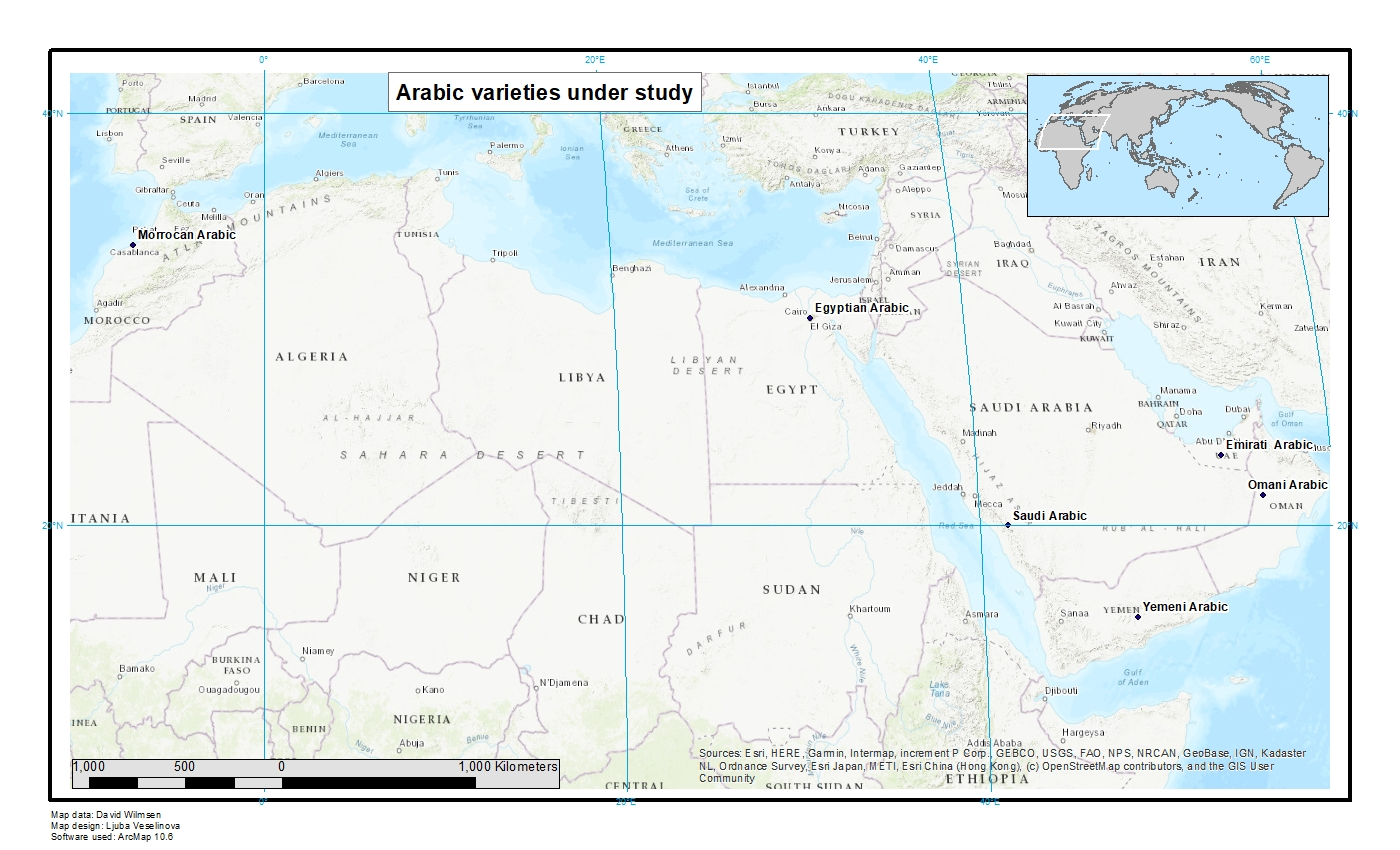
\includegraphics[width=\textwidth]{figures/Arabic_varieties_under_study_210218.jpg}
    \caption{Arabic varieties under study}
    \label{fig:ArabicVarieties}
\end{figure}



{\sloppy\printbibliography[heading=subbibliography,notkeyword=this]}

\end{document}
